\section{Experiments}
\label{sec:experiments}

\begin{table}[ht]
  \begin{tabular}{l p{0.3\textwidth} p{0.3\textwidth} r r r}
    {\bf Dataset} & {\bf Task and notes} & {\bf Features} & {\bf Init.} & {\bf Test} \\ \hline
  {\bf NER}     & 
    We evaluate on the CoNLL-2003 NER task\tablefootnote{\href{http://www.cnts.ua.ac.be/conll2003/ner/}{http://www.cnts.ua.ac.be/conll2003/ner/}}, a sequence labeling problem over English sentences. 
    We only consider the three entity tags corresponding to persons ($\textsc{per}$), locations ($\textsc{loc}$) or others ($\textsc{o}$)\tablefootnote{%
    The original also includes the tags $\textsc{org}$ and $\textsc{misc}$, however the distinctions between these tags are artificial, making it very difficult for non-expert crowd workers to provide accurate labels.}.
    &
    We used standard features~\cite{finkel2005incorporating}: the current word, current lemma, previous and next lemmas, lemmas in a window of size three to the left and right, word shape and word prefix and suffixes.
    &
  40 & 1000 \\
  {\bf Sentiment} & 
    We evaluate on the Stanford sentiment dataset that consists of 2000 polar movie reviews; task is a binary classification problem with classes $\textsc{pos}$ and $\textsc{neg}$. 
    &
    We used two feature sets, the first (\textsc{bigrams}) containing only word unigrams and bigrams, and the second (\textsc{rnn}) that also contained sentence vector embeddings from~\cite{socher2013recursive}.
    &  
  20 & 1800 \\
  {\bf Faces} & 
  We evaluate on a celebrity face classification task\tablefootnote{\todo{}}. Each image must be labeled as one of the following four choices: Andersen Cooper, Daniel Craig, Scarlet Johansson and Miley Cyrus.
    &
    We used the last layer of a 11-layer AlexNet~\cite{krizhevsky2012imagenet} trained on ImageNet as input feature embeddings.
    & 
  40 & 1784 
\end{tabular}
  \caption{Dataset used in this paper: we use a small number of elements }
\label{tbl:dataset}
%\end{table}
%\begin{table}[hb]
%% NER 
{\bf NER} \\
\begin{tabular}{l r r r r r}
    \textbf{System} & \textbf{Time/token} & \textbf{Requests/token} & \textbf{Precision} & \textbf{Recall} & \textbf{F1} \\ \hline
    Human 1-query baseline & 664 ms & 1.0 & 66.38 & 89.58 & 76.15 \\ %\hline
    Human 3-query baseline & 1495 ms & 3.0 & 92.79 & 89.56 & 91.58 \\ %\hline
    Human 5-query baseline & 3887 ms & 5.0 & 98.25 & 92.33 & 95.20 \\ %\hline
    Offline baseline & n/a & n/a & 62.38 & 69.76 & 65.86 \\ %\hline
    Threshold baseline & 1523 ms & 0.65 & 91.74 & 90.90 & 91.33 \\ %\hline
    \textbf{MCTS} & 3368 ms & \textbf{0.62} & \textbf{94.32} & \textbf{93.16} & \textbf{93.73} \\ %\hline
\end{tabular}

%% Sentimemnt
{\bf Sentiment}\\
\begin{tabular}{l  r  r  r  r}
    %\hline
    \textbf{System} & \textbf{Time/example} & \textbf{Requests/example} & \textbf{Accuracy} \\ \hline
    Human 1-query baseline & 1791 ms & 1.0 & 90.79 \\ %\hline
    Human 3-query baseline & 2478 ms & 3.0 & 92.20 \\ %\hline
    Offline baseline - Bigrams & n/a & n/a & 70.03 \\ %\hline
    Threshold baseline - Bigrams & TODO & TODO & TODO \\ %\hline
    \textbf{MCTS - Bigrams} & 2853 ms & \textbf{1.83} & \textbf{93.8} \\% \hline
    Offline baseline - RNN & n/a & n/a & 85.03 \\ %\hline
    Threshold baseline - RNN & TODO & TODO & TODO \\ %\hline
    \textbf{MCTS - RNN} & 1926 ms & \textbf{1.48} & \textbf{93.1} \\ %\hline
\end{tabular}

%% Faces
{\bf Faces}\\
\begin{tabular}{l  r  r  r  r  r}
    %\hline
    \textbf{System} & \textbf{Time/example} & \textbf{Requests/example} & \textbf{Accuracy} \\ \hline
    Human 1-query baseline & 1414 ms & 1.0 & 87.75 \\ %\hline
    Human 3-query baseline & 1865 ms & 3.0 & 88.44 \\ %\hline
    Offline baseline & n/a & n/a & 87.43 \\    %\hline
    Threshold baseline & TODO & TODO & TODO \\ %\hline
    \textbf{MCTS} & 961 ms & 1.06 & 88.45 \\   %\hline
\end{tabular}
  \caption{Top: Results on {\bf NER}, Middle: Results on {\bf Sentiment}, Bottom: Results on {\bf Faces}}
\end{table}

In this section, we empirically evaluate our approach on three datasets (\tableref{dataset}) and observe various tradeoffs on the loss function.

Each dataset set was evaluated against the following four baselines
\begin{enumerate}
  \item {\bf Human n-query}: The majority vote of $n$ human crowd workers was used as a prediction.
  \item {\bf Offline baseline}: We simulate the best possible offline system: one that can train on all the examples seen so far with gold labels to make the next prediction. The offline baseline can not query for any information about $x$.
  \item {\bf Threshold baseline}: We simulate a simple agent that is allowed to make queries on the data: for the given input, the agent queries any labels that it estimates have a marginal risk above a threshold of $0.88$, which was chosen by cross-validation. It then assumes that the uncertainity on that node has reduced by \todo{} and makes another query. This agent is allowed to ask queries but does not do any marginal inference.
  \item {\bf MCTS:} Our full system as described in \sectionref{async}.
\end{enumerate}

To initialize the models used in the offline baseline, threshold baseline and our MCTS model, we used parameters learned using a handful of examples (listed under the Init.\ column of \tableref{dataset}). 
\todo{Why did we have to initialize again?}

\paragraph{Implementation and crowdsouring setup}

We implemented our system using Amazon Mechanical Turk.
To have real time user responses, we set up a task that hired turkers on retainer. \todo{KEENON: fill up plz}.

Initially, when running experiments, we found that the results exhibited a high variance based on worker quality.
To control for the variance in worker quality across our evaluations of different methods, we collected 5 worker responses and their delays on each label ahead of time.
During simulation we sample the worker responses and delays without replacement from the frozen pool of worker responses. 
Neither MCTS nor the threshold baseline needed more than 3 queries on a single label\footnote{If accepted, we will make our datasets of frozen human responses, delays, and worker identifier tags publicly available}.

% DETAILS
% Anecdotally, we also report a range of results on 5 complete runs of our system using {\em real live crowd workers}, recruited at test time, over the first 150 sentences of our dataset. The results exhibit high variance based on worker quality.
%
%\begin{center}
%\begin{tabular}{ | r | r | r | r | r | }
%    \hline
%    Time/token & Requests/token & Precision & Recall & F1 \\ \hline
%    1444 ms - 3426 ms & 0.54 - 0.66 & 92.9 - 96.91 & 82.50 - 94.01 & 87.4 - 95.43 \\ \hline
%\end{tabular}
%\end{center}
%
%Filtering workers while running, or inferring separate error models for each worker, would clearly deliver substantial gains in reliability over a system that assumes uniform quality. We leave this to future work.

\todo{Keenon: Briefly brag about how excellent our results are on different datasets.}

We report results under two different sets of features: \{unigrams, bigrams\}, and \{unigrams, bigrams, Socher et al recursive sentence embeddings\todo{cite}\}. The comparison is designed to highlight that given a more powerful feature representation, our system is able to achieve higher accuracies for lower cost. Better modelling is not required to get high performance, as a higher spending rate can achieve that, but it does improve the achievable points on the cost-precision tradeoff curve.


\paragraph{Does the model learn with time?} 
\figureref{ner-running-f1}
The first thing to verify is that our system is producing consistently high accuracy, despite having a very small number of
training examples. This plot shows the F1 of the classifier, on all sentences seen 
so far, plotted at every sentence.
The x-axis is number of sentences seen, and the y-axis is F1 on those sentences.

\begin{figure}[t]
  \begin{centering}
  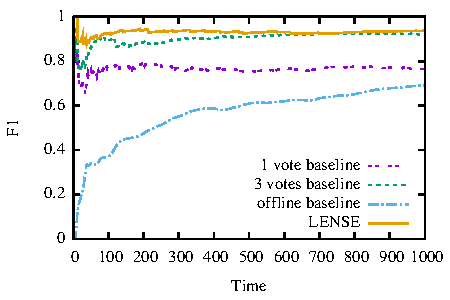
\includegraphics[width=1.0\textwidth]{figures/ner_2_class/f1_plot/f1_vs_time.pdf}
  \end{centering}
  \caption{A figure showing the comparative F1 vs time of several real-time regimes. The purple line is our system, costing just 0.65 queries per token. The green line is the 3-vote human baseline, costing 3 queries per token. The red line is the 1-vote baseline. The blue line is the performance of our classifier on its own, if we didn't allow it to query humans, and only gave it gold labels after classification in order to train.}
\label{fig:ner-running-f1}
\end{figure}

%The key takeaway is that our customers are receiving uninterupted, high quality service, and are completely unaware that throughout the experiment our classifier has too little data to generalize well by itself.

\paragraph{Does our model improve over time?}
It is obvious that given human inputs on each example, our model will do well.
However, the system has the capability of learning on-the-job.
See \figureref{ner-cost}

The third thing to verify is that our querying behavior is sound.
We don't want to see uniform querying, because that means the system isn't taking advantage of the information in our learned prior.
We also want to see a slight decrease over time, consistent with maintaining high accuracy rates.
This graph plots our queries per sentence on each iteration, normalized by sentence length.

\begin{figure}[t]
  \begin{centering}
  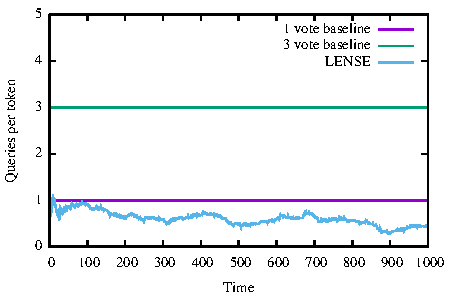
\includegraphics[width=1.0\textwidth]{figures/ner_2_class/cost_plot/cost_vs_time.pdf}
  \end{centering}
  \caption{A figure showing the number of queries required by our system, the 1 and 3 human query baselines over time.}
\label{fig:ner-cost}
\end{figure}

This plot shows two things. First, there is high variance between sentences on how many queries are needed.
Many sentences come in with such a strong prior that they can be immediately classified, with no need to ask humans.
When querying does take place, it is generally directed towards uncertain tokens.



We receive far less supervision than in the general case.
However, to reduce the costs in the future, our system must learn to generalize well.
\figureref{ner-dev-f1}
The second thing to verify is that we are training a good classifier over time. We held out a dev set of 300 sentences from
the CoNLL NER data that we didn't test on (ie in addition to the 1000 sentences we ran the system on). Every time we retrained
our classifier, we ran it on the this held out dev set, and plot F1. This is to demonstrate that, as expected, we can see
significant improvements in the classifier performance as soon as 1000 sentences in.

\begin{figure}[t]
  \begin{centering}
  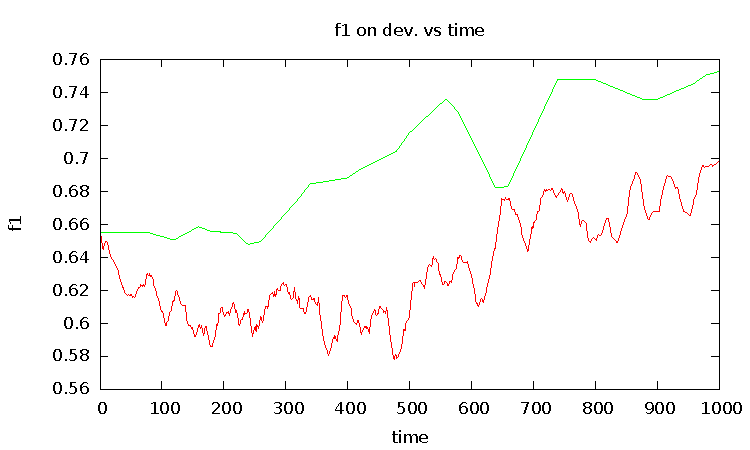
\includegraphics[width=1.0\textwidth]{figures/ner_2_class/machine_f1_plot/machine_f1_vs_time.pdf}
  \end{centering}
  \caption{A figure showing the relationship between the classifier we train, and one trained on gold labeled data. Evaluation is on a held out dev set. Note that our classifier learns more slowly because we are handing it a noisy approximation to train on, but the classifier narrows the gap as it gets more data.}
\label{fig:ner-dev-f1}
\end{figure}

Here the key takeaway is that even though the data we're training this classifier on introduces some noise (we never see
ground truth, just our guesses based on human observations), we are still improving our model from 65 to 70 f1 over the course
of only 1000 examples.

\todo{KEENON: Compare against baseline classifiers}

\paragraph{When does the model query?}

As a representative example of this querying behavior from the set, take observed behavior when tagging the sentence:

\begin{center}
\textit{``U.S.\ says still committed to Cuba migration pacts.''}
\end{center}

The system, having never seen the token before, starts with a belief that Cuba is 59\% Person, 37\% Location, and 3\% None. The system knows already, from previously learned examples, that ``U.S.'' is a Location with 97\% probability. It immediately fires off two queries about ``Cuba,'' and waits 4 seconds for both responses to return Location. It now believes that ``Cuba'' is a Location with 95\% probability, and decides to turn in its current guess. This guess is added to the training set, and the model is updated.

\paragraph{How do model features change accuracy?}

This is a graph of the relative cost per example over time, for the basic features (green) and the rich RNN embedding features (red):

\begin{figure}[t]
  \begin{centering}
  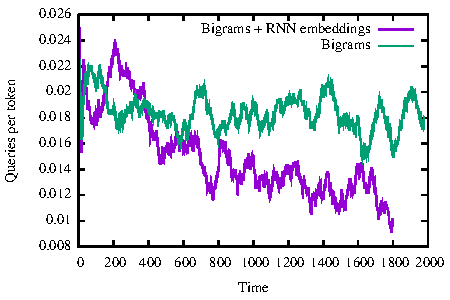
\includegraphics[width=1.0\textwidth]{figures/sentiment_cost_per_token_vs_time/cost_per_token_vs_time.pdf}
  \end{centering}
  \caption{A figure showing that increasing model capacity with richer distributional features (red line) enables the model to reduce costs further over time, compared with a simpler bag-of-words model with less representational capacity (green line).}
\label{fig:crf}
\end{figure}

The thing to note is that although accuraccy rates remain high for both approaches throughout, the richer model is able to learn more over time, and subsequently costs the operator of our system less.
Something about model capacity.

